\documentclass[12pt,letterpaper]{article}
\usepackage{graphicx,textcomp}
\usepackage{natbib}
\usepackage{setspace}
\usepackage{fullpage}
\usepackage{color}
\usepackage[reqno]{amsmath}
\usepackage{amsthm}
\usepackage{fancyvrb}
\usepackage{amssymb,enumerate}
\usepackage[all]{xy}
\usepackage{endnotes}
\usepackage{lscape}
\newtheorem{com}{Comment}
\usepackage{float}
\usepackage{hyperref}
\newtheorem{lem} {Lemma}
\newtheorem{prop}{Proposition}
\newtheorem{thm}{Theorem}
\newtheorem{defn}{Definition}
\newtheorem{cor}{Corollary}
\newtheorem{obs}{Observation}
\usepackage[compact]{titlesec}
\usepackage{dcolumn}
\usepackage{tikz}
\usetikzlibrary{arrows}
\usepackage{multirow}
\usepackage{xcolor}
\newcolumntype{.}{D{.}{.}{-1}}
\newcolumntype{d}[1]{D{.}{.}{#1}}
\definecolor{light-gray}{gray}{0.65}
\usepackage{url}
\usepackage{listings}
\usepackage{color}
\usepackage{booktabs}
\definecolor{codegreen}{rgb}{0,0.6,0}
\definecolor{codegray}{rgb}{0.5,0.5,0.5}
\definecolor{codepurple}{rgb}{0.58,0,0.82}
\definecolor{backcolour}{rgb}{0.95,0.95,0.92}
\usepackage{booktabs}
\usepackage{caption}
\usepackage{graphicx}

\lstdefinestyle{mystyle}{
	backgroundcolor=\color{backcolour},   
	commentstyle=\color{codegreen},
	keywordstyle=\color{magenta},
	numberstyle=\tiny\color{codegray},
	stringstyle=\color{codepurple},
	basicstyle=\footnotesize,
	breakatwhitespace=false,         
	breaklines=true,                 
	captionpos=b,                    
	keepspaces=true,                 
	numbers=left,                    
	numbersep=5pt,                  
	showspaces=false,                
	showstringspaces=false,
	showtabs=false,                  
	tabsize=2
}
\lstset{style=mystyle}
\newcommand{\Sref}[1]{Section~\ref{#1}}
\newtheorem{hyp}{Hypothesis}

\begin{document}
\maketitle
	\section*{Legacies of Wartime Order: Punishment Attacks and Social Control in Northern Ireland by Kit Rickard & Kristin M. Bakke }
	
	Jacqueline Bouvier SN 23364975
\section*{Main Themes/Questions}
The study speaks to broader debates about governance, the rule of law, and state-society relations. Informal institutions that have emerged in wartime have a legacy that continues past wartime agreements and treaties. The social control from these institutions grips communities because both armed actors and civilians hold a certain reliance on them. Many post-conflict societies have the emergence of non-state armed groups that can minimize the credibility of a state. The determining factors of why the hold is so great on the communities vary from fear to not being able to trust or rely on the formal institutions.

The informal justice systems created during the Troubles in Northern Ireland by both Catholic and Protestant sides have held a grip on their communities past the signing of the Good Friday Agreement in 1998. A main function of these groups is an informal justice system that would serve to punish those who acted out in the community.
\section*{Hypothesis}
\begin{itemize}
\item Assessing whether paramilitary groups’ social control during the Troubles is associated with the location of paramilitary-style attacks today while also accounting for other variables that can account for the occurrence of such attacks today, not least deprivation.
\item Civilians rely on informal justice institutions persist into the post conflict period due to mistrust of police.
\end{itemize}
\section*{Data}
With the use of a dataset of geolocated paramilitary-style attacks (PSAs) from the Police Service of Northern Ireland (PSNI) and interviews, statistical analysis was performed to examine the following with the PSNI data:
\begin{itemize}
	\item Logit Model – examine whether in-group killings from the Troubles are associated with paramilitary-style attacks (post-conflict)
	\item Negative Binomial – examine whether in-group killings are associated with the intensity of post-conflict paramilitary-style attacks.
\end{itemize}

\textbf{Dependent Variables:} Republican PSAs, Loyalist PSAs \\
\textbf{Independent Variables:} Catholic in-group killings (1969-1998), Protestant in-group killings (1969-1998), Total population, Urban, Catholic stronghold, Protestant stronghold, Income deprivation rate, Violent crime rate, Anti-social behavior rate

With the following from the surveys, three logistic regression models were run:
\begin{itemize}
	\item Whether respondents rate the police as effective
	\item Whether respondents rate the informal authorities effective
	\item Whether respondents rate the effectiveness of the informal authorities as higher than the police.
\end{itemize}

\textbf{Dependent Variables:} Catholic respondents, Protestant respondents \\
\textbf{Independent Variables:} Republican PSA, Loyalist PSA, Age, Male, General Trust, Trust in neighborhood, Discriminated, Victim of state violence (1969-1998), Community Stronghold, Income deprivation, Urban.
\section*{Conclusion}
The models produced show that the associations between the paramilitary groups social control and people perceptions post war of formal and informal authoritites. It can be assumed that the results show a more top-down and incentive but also a bottom up, a fear and respect verse coercion. When breaking down between Catholic and Protestant respondents we can see a pattern of skepticism of formal authorities from Catholics and a positive view of effectiveness of informal authorities among Protestants. This goes inline with findings from the Independent Reporting Commission from 2018 that fear and anger about continuation of informal authorities but also were regarded as protectors. 

The study suggests possible scopes for future works on informal institutions and legacys of informal war time institutions. State building that goes on postwar doesn't necessarily happen in a governance vacuum and these institutions may exisit due to the emphasis of a more "socio" side of paramilitary control. 
	\lstinputlisting[language=R, firstline=12, lastline=12]{replication.R}]
		\lstinputlisting[language=R, firstline=72, lastline=74]{replication.R}]

\newpage
\section*{Table 1}
		\lstinputlisting[language=R, firstline=14, lastline=40]{replication.R}]
	
	\begin{table}[htbp]
		\centering
		\caption{Logistic Regression Models for Paramilitary-style Assaults (2016-2018)}
		\begin{tabular}{lcc}
			\toprule
			& \textbf{Republican PSAs} & \textbf{Loyalist PSAs} \\
			\midrule
			\textbf{Catholic in-group killings (1969-1998)} & 0.27*** & \\
			& (0.07) & \\
			\textbf{Protestant in-group killings (1969-1998)} & & 0.45*** \\
			& & (0.13) \\
			\textbf{Total population} & 0.23 & 0.16 \\
			& (0.17) & (0.13) \\
			\textbf{Urban} & 1.99** & 1.10*** \\
			& (0.63) & (0.33) \\
			\textbf{Catholic stronghold} & 1.78*** & \\
			& (0.36) & \\
			\textbf{Protestant stronghold} & & 1.61*** \\
			& & (0.26) \\
			\textbf{Income deprivation rate} & 12.54** & 10.76** \\
			& (4.54) & (3.55) \\
			\textbf{Violent crime rate} & 0.02 & -0.04* \\
			& (0.02) & (0.02) \\
			\textbf{Anti-social behavior rate} & -0.01 & 0.03** \\
			& (0.01) & (0.01) \\
			\midrule
			\textbf{AIC} & 289.42 & 529.60 \\
			\textbf{BIC} & 327.75 & 567.93 \\
			\textbf{Log Likelihood} & -136.71 & -256.80 \\
			\textbf{Deviance} & 273.42 & 513.60 \\
			\textbf{Num. obs.} & 890 & 890 \\
			\bottomrule
		\end{tabular}
		\label{tab:logistic_regression}
		\medskip
		\small
		\raggedright
		Notes: *** p < 0.001, ** p < 0.01, * p < 0.05. Analysis conducted in R.
	\end{table}
	\newpage
\section*{Table 2}
	\lstinputlisting[language=R, firstline=42, lastline=68]{replication.R}]
	
	\begin{table}[htbp]
		\centering
		\caption{Negative Binomial Models for PSAs (2016-2018)}
		\begin{tabular}{lcc}
			\toprule
			& \textbf{Republican PSAs} & \textbf{Loyalist PSAs} \\
			\midrule
			\textbf{Catholic in-group killings (1969-1998)} & 0.15** & \\
			& (0.05) & \\
			\textbf{Protestant in-group killings (1969-1998)} & & 0.18* \\
			& & (0.08) \\
			\textbf{Total population} & 0.18 & 0.17 \\
			& (0.16) & (0.12) \\
			\textbf{Urban} & 1.57** & 0.97** \\
			& (0.51) & (0.31) \\
			\textbf{Catholic stronghold} & 2.18*** & \\
			& (0.33) & \\
			\textbf{Protestant stronghold} & & 1.41*** \\
			& & (0.24) \\
			\textbf{Income deprivation rate} & 7.72* & 8.80** \\
			& (3.88) & (3.18) \\
			\textbf{Violent crime rate} & 0.04** & -0.03 \\
			& (0.02) & (0.01) \\
			\textbf{Anti-social behavior rate} & -0.02* & 0.03*** \\
			& (0.01) & (0.01) \\
			\midrule
			\textbf{AIC} & 423.56 & 741.21 \\
			\textbf{BIC} & 466.68 & 784.33 \\
			\textbf{Log Likelihood} & -202.78 & -361.60 \\
			\textbf{Deviance} & 192.83 & 337.53 \\
			\textbf{Num. obs.} & 890 & 890 \\
			\bottomrule
		\end{tabular}
		\label{tab:negative_binomial}
		\medskip
		\small
		\raggedright
		Notes: *** p < 0.001, ** p < 0.01, * p < 0.05. Analysis conducted in R.
	\end{table}
	\newpage
\section*{Table 3}
	\lstinputlisting[language=R, firstline=75, lastline=83]{replication.R}]
	
\begin{table}[htbp]
	\centering
	\caption{Respondents' view of the effectiveness of contacting "the police"}
	\resizebox{\linewidth}{!}{%
		\begin{tabular}{lccc}
			\toprule
			& \textbf{All respondents} & \textbf{Catholic respondents} & \textbf{Protestant respondents} \\
			\midrule
			This would make no difference (\%) & 17 & 20 & 15 \\
			This might help a little (\%) & 46 & 47 & 46 \\
			This would help a lot (\%) & 34 & 30 & 38 \\
			"Don't know" or refused to answer (\%) & 2 & 3 & 1 \\
			\bottomrule
		\end{tabular}%
	}
	\label{tab:police_effectiveness}
\end{table}
\newpage
\section*{Table 4}
	\lstinputlisting[language=R, firstline=87, lastline=95]{replication.R}]

\begin{table}[htbp]
	\centering
	\caption{Respondents' view of the effectiveness of contacting "a member of the community who has influence"}
	\resizebox{\linewidth}{!}{%
		\begin{tabular}{lccc}
			\toprule
			& \textbf{All respondents} & \textbf{Catholic respondents} & \textbf{Protestant respondents} \\
			\midrule
			This would make no difference (\%) & 19 & 19 & 18 \\
			This might help a little (\%) & 48 & 48 & 47 \\
			This would help a lot (\%) & 28 & 26 & 32 \\
			"Don't know" or refused to answer (\%) & 6 & 7 & 4 \\
			\bottomrule
		\end{tabular}%
	}
	\label{tab:community_influence}
\end{table}
\newpage
\section*{Table 5}
	\lstinputlisting[language=R, firstline=99, lastline=123]{replication.R}]
	\begin{table}[htbp]
		\centering
		\caption{Respondents' rating of police as effective when faced with an anti-social behavior scenario}
		\begin{tabular}{lcc}
			\toprule
			& \textbf{Catholic respondents'} & \textbf{Protestant respondents'} \\
			\midrule
			Republican PSAs             & -0.19** & \\
			& (0.07) & \\
			Loyalist PSAs               & & -0.04 \\
			& & (0.09) \\
			Age                         & -0.00 & 0.00 \\
			& (0.01) & (0.01) \\
			Male                        & -1.04*** & 0.27 \\
			& (0.30) & (0.30) \\
			General trust               & -0.39 & -0.78* \\
			& (0.32) & (0.33) \\
			Trust in neighbourhood     & 0.39 & 0.39 \\
			& (0.23) & (0.25) \\
			Income deprivation (SOA)   & -0.02 & -9.18* \\
			& (4.22) & (4.36) \\
			\midrule
			AIC                         & 320.45 & 332.86 \\
			BIC                         & 362.34 & 376.74 \\
			Log Likelihood              & -149.23 & -155.43 \\
			Deviance                    & 298.45 & 310.86 \\
			Num. obs.                   & 333 & 399 \\
			\bottomrule
		\end{tabular}
		\label{tab:model_comparison}
		\medskip
		\small
		\raggedright
		Notes: *** p < 0.001, ** p < 0.01, * p < 0.05.
	\end{table}
	\newpage
	\section*{Table 6}
		\lstinputlisting[language=R, firstline=127, lastline=152]{replication.R}]
	
	\begin{table}[htbp]
		\centering
		\caption{Respondents' rating of informal authorities as effective when faced with an anti-social behavior scenario}
		\begin{tabular}{lcc}
			\toprule
			& \textbf{Catholic respondents'} & \textbf{Protestant respondents'} \\
			\midrule
			Republican PSAs             & -0.05 & \\
			& (0.07) & \\
			Loyalist PSAs               & & 0.30* \\
			& & (0.13) \\
			Age                         & -0.01 & 0.01 \\
			& (0.01) & (0.01) \\
			Male                        & 0.11 & -0.16 \\
			& (0.30) & (0.28) \\
			General trust               & 0.95** & -0.02 \\
			& (0.33) & (0.29) \\
			Trust in neighbourhood     & 0.92*** & 0.22 \\
			& (0.25) & (0.24) \\
			Income deprivation (SOA)   & -0.16 & -14.40*** \\
			& (4.23) & (4.16) \\
			\midrule
			AIC                         & 312.79 & 366.68 \\
			BIC                         & 354.25 & 410.20 \\
			Log Likelihood              & -145.40 & -172.34 \\
			Deviance                    & 290.79 & 344.68 \\
			Num. obs.                   & 320 & 386 \\
			\bottomrule
		\end{tabular}
		\label{tab:informal_authorities}
		\medskip
		\small
		\raggedright
		Notes: *** p < 0.001, ** p < 0.01, * p < 0.05.
	\end{table}
	\newpage
	\section*{Table 7}
		\lstinputlisting[language=R, firstline=155, lastline=180]{replication.R}]
	
	\begin{table}[htbp]
		\centering
		\caption{Respondents' rating of informal authorities as more effective than the police when faced with an anti-social behavior scenario}
		\begin{tabular}{lcc}
			\toprule
			& \textbf{Catholic respondents'} & \textbf{Protestant respondents'} \\
			\midrule
			Republican PSAs             & 0.03 & \\
			& (0.06) & \\
			Loyalist PSAs               & & 0.25** \\
			& & (0.08) \\
			Age                         & -0.00 & 0.01 \\
			& (0.01) & (0.01) \\
			Male                        & 0.18 & -0.06 \\
			& (0.27) & (0.25) \\
			General trust               & 1.00*** & 0.47 \\
			& (0.30) & (0.26) \\
			Trust in neighbourhood     & -0.19 & -0.25 \\
			& (0.21) & (0.22) \\
			Income deprivation (SOA)   & -1.13 & -10.01** \\
			& (3.79) & (3.86) \\
			\midrule
			AIC                         & 366.60 & 429.79 \\
			BIC                         & 407.99 & 473.31 \\
			Log Likelihood              & -172.30 & -203.90 \\
			Deviance                    & 344.60 & 407.79 \\
			Num. obs.                   & 318 & 386 \\
			\bottomrule
		\end{tabular}
		\label{tab:informal_authorities_comparison}
		\medskip
		\small
		\raggedright
		Notes: *** p < 0.001, ** p < 0.01, * p < 0.05.
	\end{table}
	\newpage
	\section*{Figure1}
	\lstinputlisting[language=R, firstline=186, lastline=221]{replication.R}]
\begin{figure}[htbp]
	\centering
	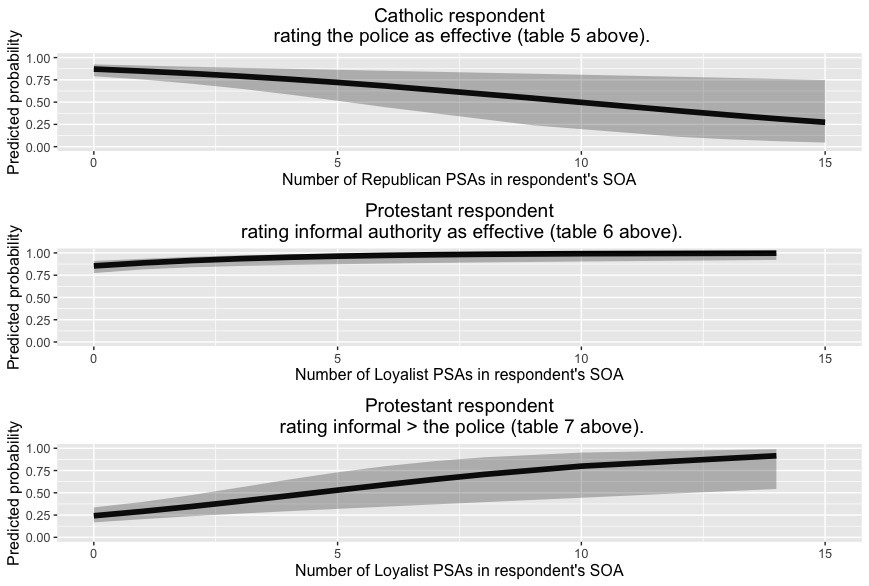
\includegraphics[width=\textwidth]{figure1.jpeg}
	\caption{Predicted probabilities for the statistically significant results from the models reported in tables 5, 6, and 7. All variables are set at their mean or mode.}
	\label{fig:predicted_probabilities}
\end{figure}


\end{document}